% vim: set textwidth=78 autoindent:

\section{Integrazione con GRASS GIS}\label{sec:grass}\index{GRASS}

% when the revision of a section has been finalized, 
% comment out the following line:
%\updatedisclaimer

Il plugin GRASS consente l'accesso ai dati e alle funzioni di GRASS
GIS~\cite{GRASSweb}, inclusa la visualizzazione di layer raster e vettoriali,
la digitalizzazione di layer vettoriali, la modifica degli attributi e la
creazione di nuovi vettori, e l'analisi di dati GRASS 2D e 3D tramite più di
300 moduli GRASS.

In questa Sezione verranno forniti un'introduzione sulle funzionalità del plugin
e qualche esempio sulla gestione e l'utilizzo di dati GRASS. Quando viene
abilitato il plugin GRASS come descritto alla Sezione~\ref{sec:starting_grass},
nella barra sono disponibili i seguenti strumenti:
 
\begin{itemize}
\item \toolbtntwo{grass_open_mapset}{Apri mapset}
\item \toolbtntwo{grass_new_mapset}{Nuovo mapset}
\item \toolbtntwo{grass_close_mapset}{Chiudi mapset}
\item \toolbtntwo{grass_add_vector}{Aggiungi vettoriale GRASS}
\item \toolbtntwo{grass_add_raster}{Aggiungi raster GRASS}
\item \toolbtntwo{grass_new_vector_layer}{Crea nuovo vettoriale GRASS}
\item \toolbtntwo{grass_edit}{Modifica vettoriale GRASS}
\item \toolbtntwo{grass_tools}{Apri strumenti GRASS}
%\item \toolbtntwo{grass_shell}{Open GRASS Shell}
\item \toolbtntwo{grass_region}{Visualizza GRASS regione attuale} 
\item \toolbtntwo{grass_region_edit}{Modifica region GRASS attuale}
\end{itemize}

\subsection{Avviare il plugin GRASS}\label{sec:starting_grass}
\index{GRASS!avviare da QGIS}

Per usare le funzioni GRASS e/o visualizzare layer raster e vettoriali in
formato GRASS in QGIS, bisogna prima selezionare e caricare il plugin GRASS con il
QGIS Plugin Manager. 
Cliccare quindi sul menu \mainmenuopt{Plugins} > \mainmenuopt{Gestione plugin}, 
selezionare \dropmenuopt{GRASS} e cliccare \button{OK}. 

Ora è possibile caricare layer raster e vettoriali da una \filename{LOCATION}
GRASS esistente (si veda la Sezione \ref{sec:load_grassdata}). È anche
possibile creare una nuova \filename{LOCATION} GRASS in QGIS (si veda la
Sezione \ref{sec:create_loc}) e importarci dati raster e vettoriali (si
veda la Sezione \ref{sec:import_loc_data}) per ulteriori analisi con gli
strumenti GRASS (si veda la Sezione \ref{subsec:grass_toolbox}).

\subsection{Caricare layer raster e vettoriali GRASS}\label{sec:load_grassdata}\index{GRASS!caricamento dati}

Con il plugin GRASS, possono essere caricati layer raster o vettoriali
usando il pulsante appropriato nella barra strumenti. Come esempio si
consideri il set di dati Alaska (si veda la Sezione \ref{label_sampledata}).
Esso include un piccolo \filename{LOCATION} GRASS campione contenente tre layer
vettoriali e una mappa di altitudine raster.

\begin{enumerate}
  \item Creare una nuova cartella \filename{grassdata}, nella quale scaricare
  il set di dati Alaska denominato \filename{qgis\_sample\_data.zip}
  dall'indirizzo web \url{http://download.osgeo.org/qgis/data/} e decomprimere
  il file nella cartella \filename{grassdata}.
  \item Avviare QGIS.
  \item Se non è già stato fatto in precedenti sessioni di QGIS, caricare il
  plugin GRASS cliccando su\mainmenuopt{Plugins} > \mainmenuopt{Gestione
  Plugin} e selezionare \dropmenuopt{GRASS}. La barra GRASS apparirà nella
  barra strumenti.
  \item Nella barra strumenti GRASS, cliccare sull'icona
  \toolbtntwo{grass_open_mapset}{Apri mapset} per aprire la finestra
  \filename{Seleziona Mapset}.
  \item Alla voce \filename{Gisdbase} inserire l'indirizzo completo o navigare
  fino alla cartella \filename{grassdata} appena creata.
  \item Dovrebbe ora essere possibile selezionare la \filename{LOCATION
  alaska} e il MAPSET \filename{demo}. 
  \item Cliccare su \button{OK}. Si noti che ora alcuni degli strumenti
  precedentemente disabilitati sono divenuti attivi.
  \item Cliccare su \toolbtntwo{grass_add_raster}{Aggiungi raster GRASS},
  scegliere la mappa denominata \filename{gtopo30} e cliccare su \button{OK}.
  Verrà visualizzato il layer delle elevazioni del terreno.
  \item Cliccare su \toolbtntwo{grass_add_vector}{Aggiungi vettoriale GRASS},
  selezionare la mappa denominata \filename{alaska} e cliccare su \button{OK}.
  Il confine dell'Alaska verrà sovrapposto alla mappa gtopo30 map. Ora è
  possibile adattare le proprietà del layer come descritto al capitolo
  \ref{sec:vectorprops}, ovvero cambiare la trasparenza, il colore di
  riempimento e del contorno dell'elemento.
  \item Caricare anche gli altri due layer vettoriali denominati
  \filename{rivers} e \filename{airports} e modificarne le proprietà.
\end{enumerate}

Come dimostrato è quindi molto semplice caricare dati raster e vettoriali in
formato GRASS in QGIS. Si veda la sezione seguente per sapere come editare
dati GRASS e creare nuove \filename{LOCATION}. Ulteriori \filename{LOCATIONs}
campione di GRASS sono disponibili sul siti di GRASS all'indirizzo
\url{http://grass.osgeo.org/download/data.php}.

\begin{Tip}\caption{\textsc{Caricare dati GRASS}}
\qgistip{Se si presentano problemi nel caricare dati o QGIS termina
inaspettatamente, assicurarsi di aver caricato il plugin GRASS correttamente
come descritto alla Sezione \ref{sec:starting_grass}.
}
\end{Tip} 

\subsection{LOCATION e MAPSET in GRASS}\label{sec:about_loc}

GRASS organizza i propri in cartelle alle quali si fa riferimento con la
denominazione GISDBASE. Queste cartelle, spesso chiamate \filename{grassdata},
devono essere create prima di iniziare a lavorare con il plugin GRASS in QGIS.
In queste directory, i dati GRASS sono organizzati per progetti inseriti in
sottocartelle chiamate \filename{LOCATION}. 
Ogni \filename{LOCATION} è definita da un sistema di coordinate, da un sistema
di proiezione e dall'estensione geografica. La \filename{LOCATION} può avere a
sua volta molte sottocartelle \filename{MAPSETs} usate per suddividere il
progetto in diversi argomenti, sottoregioni o spazi di lavoro per i diversi
membri del team che vi sta lavorando (Neteler \& Mitasova 2008
\cite{neteler_mitasova08}). Per analizzare layer raster e vettoriali con i
moduli GRASS, bisogna importarli in una \filename{LOCATION} GRASS.
\footnote{Questo non è proprio vero - con i moduli GRASS \filename{r.external}
e \filename{v.external} è possibile creare collegamenti in sola lettura ai
dati GDAL/OGR supportati senza che sia necessario effettuare l'importazione.
Tuttavia siccome questa non è la modalità predefinita per i principianti
questa funzione non verrà descritta.}

\begin{figure}[ht]
\begin{center}
\caption{Organizzazzione dei dati GRASS nella LOCATION campione alaska
(adattato da Neteler \& Mitasova 2008 \cite{neteler_mitasova08})}\label{fig:grass_location}\smallskip

\includegraphics[clip=true]{grass_location}
\end{center}  
\end{figure}

\subsubsection{Creare una nuova LOCATION GRASS}\label{sec:create_loc}

Per questo e per tutti i successivi esempi riguardanti GRASS GIS verrà usata la \filename{LOCATION
alaska} campione, che è proiettata nel sistema Albers Equal Area con unità di
misura in metri, creata dal set di dati campione di QGIS. Sarà utile scaricare
ed installare il set di dati sul proprio computer \ref{label_sampledata}).

\begin{figure}[ht]
\begin{center}
\caption{Creazione di una nuova LOCATION GRASS o di un nuovo MAPSET in QGIS \nixcaption}
\label{fig:create_grass_location}\smallskip
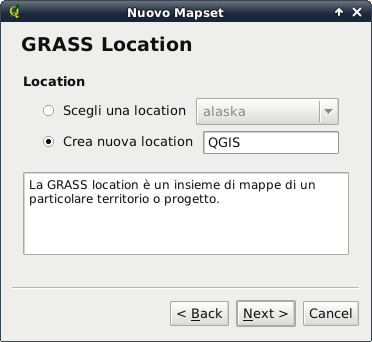
\includegraphics[clip=true, width=10cm]{create_grass_location}
\end{center}  
\end{figure}

\begin{enumerate}
  \item Avviare QGIS e assicurarsi che il plugin GRASS sia caricato
  \item Visualizzare lo shapefile \filename{alaska.shp} (si veda la Sezione
  \ref{sec:load_shapefile}) dal set di dati alaska~\ref{label_sampledata}.
  \item Nella barra strumenti GRASS, cliccare sull'icona
  \toolbtntwo{grass_new_mapset}{Nuovo mapset} per avviare la procedura guidata.
  \item Selezionare la cartella contenente il database GRASS (GISDBASE)
  denominata \filename{grassdata} o crearne una nuova in cui ospitare la nuova
  \filename{LOCATION} usando il gestore di file installato sul proprio
  computer. Cliccare su \button{Next}. 
  \item Per creare un nuovo \filename{MAPSET} in una \filename{LOCATION}
  esistente (si veda la Sezione~\ref{sec:add_mapset}) o per creare una nuova
  \filename{LOCATION}, selezionare l'opzione \radiobuttonon{Crea nuova
  location} (si veda la Figura \ref{fig:create_grass_location}).
  \item Inserire il nome della \filename{LOCATION} - nell'esempio abbiamo
  usato alaska, e cliccare su \button{Next} 
  \item Definire la proiezione cliccando sull'opzione
  \radiobuttonon{Proiezione} per abilitare l'elenco delle proiezioni 
  \item Scegliere la proiezione Albers Equal Area Alaska (feet). Siccome ne
  conosciamo l'identificativo EPSG che è 2964, inserirlo nella casella di
  ricerca. (Nota: se si vuole ripetere il processo per un'altra
  \filename{LOCATION} e non si è memorizzato l'identificativo EPSG della
  proiezione, cliccare sull'icona   \toolbtntwo{mIconProjectionEnabled}{Stato CRS}
  nella parte destra inferiore della barra di stato (si veda la sezione \ref{label_projstart})).
  \item Cliccare su \button{Trova} per selezionare la proiezione
  \item Cliccare su \button{Next} 
  \item Per definire l'estensione della regione di default, bisogna inserire i
  limiti della \filename{LOCATION} verso nord, sud, est e ovest. Nel nostro
  esempio cliccare semplicemente sul pulsante \button{Imposta estensione
  attuale di QGIS}, per applicare l'estensione del layer caricato
  \filename{alaska.shp} come estensione di default della region GRASS.
  \item Cliccare su \button{Next} 
  \item Abbiamo anche bisogno di definire un \filename{MAPSET} interno alla
  location \filename{LOCATION}. Il nome è a scelta, nell'esempio abbiamo
  usato demo.
  \footnote{Quando si crea una nuova \filename{LOCATION}, GRASS crea
  automaticamente un \filename{MAPSET} speciale chiamato \filename{PERMANENT}
  designato a contenere i dati di base del progetto, l'estensione spaziale di
  default e la definizione del sistema di coordinate (Neteler \& Mitasova 2008 
  \cite{neteler_mitasova08}).}
  \item Controllare il riassunto per assicurarsi che le impostazioni siano
  corrette e cliccare su \button{Finish} 
  \item La nuova \filename{LOCATION alaska} e i \filename{MAPSETs demo}
  e \filename{PERMANENT} vengono creati. Il set di lavoro impostato per il
  lavoro corrente è il \filename{MAPSET demo}.
  \item Si noti che alcuni strumenti della barra di GRASS precedentemente
  disabilitati sono ora attivi.
\end{enumerate}

Per quanto possa essere apparsa lunga, questa procedura costituisce un modo
veloce per creare una \filename{LOCATION}. La \filename{LOCATION alaska} è ora
pronta per l'importazione dei dati (si veda la Sezione \ref{sec:import_loc_data}).
È anche possibile usare dati raster e vettoriali esistenti nella
\filename{LOCATION alaska} campione in formato GRASS inclusi nel dataset
alaska di QGIS \ref{label_sampledata} e procedere alla Sezione \ref{label_vectmodel}.

\subsubsection{Aggiungere un nuovo MAPSET}\label{sec:add_mapset}

Ogni utente ha accesso in scrittura solo ai \filename{MAPSET} GRASS che ha
creato. Ciò implica che oltre ad accedere ai propri \filename{MAPSET},
l'utente può anche leggere i dati contenuti nei \filename{MAPSETs} creati da
altri, ma può modificare o rimuovere solo i dati nei suoi \filename{MAPSET}.
Tutti i \filename{MAPSETs} includono un file denominato \filename{WIND} nel
quale sono immagazzinati i valori di coordinate dei limiti della regione
impostata e la risoluzione spaziale impostata per i raster (Neteler \& Mitasova 2008
\cite{neteler_mitasova08}, si veda la Sezione \ref{sec:grass_region}). 
Per creare un nuovo \filename{MAPSET}:

\begin{enumerate}
  \item Avviare QGIS e assicurarsi che il plugin GRASS sia abilitato
  \item Nella barra strumenti GRASS, cliccare sull'icona
  \toolbtntwo{grass_open_mapset}{Apri mapset} per aprire la procedura guidata
  di creazione del \filename{MAPSET}.
  \item Selezionare la cartella GRASS (GISDBASE) \filename{grassdata} con il
  nome \filename{LOCATION alaska}, nel quale si vuole aggiungere un ulteriore
  \filename{MAPSET}, che chiameremo test.
  \item Cliccare su \button{Next}. 
  \item Con questa procedura possiamo creare un nuovo \filename{MAPSET}
  all'interno di una \filename{LOCATION} esistente i creare anche una nuova
  \filename{LOCATION} contemporaneamente. Cliccare sull'opzione
  \radiobuttonon{Selezionare location} (si veda la Figura
  \ref{fig:create_grass_location}) e cliccare su \button{Next}.
  \item Inserire il nome \filename{test} per il nuovo \filename{MAPSET}. Più
  sotto nella finestra è visibile una lista di \filename{MAPSETs} esistenti e
  i relativi proprietari.
  \item Cliccare su \button{Next}, controllare che il riassunto per
  assicurarsi che le impostazioni siano corrette e cliccare \button{Finish}.
\end{enumerate}

\subsection{Importare dati nelle LOCATION GRASS}\label{sec:import_loc_data}

Questa Sezione fornisce un esempio su come importare dati raster e vettoriali
nella \filename{LOCATION} GRASS \filename{alaska} fornita dal set di dati QGIS
alaska. Verrà usata la mappa raster dell'uso del suolo \filename{landcover.img} e
il vettoriale poligonale denominato \filename{lakes.gml} dal set di dati
medesimo \ref{label_sampledata}.

\begin{enumerate}
  \item Avviare QGIS e assicurarsi che il plugin GRASS sia caricato.
  \item Nella barra strumenti GRASS, cliccare sull'icona
  \toolbtntwo{grass_open_mapset}{Open MAPSET} per avviare la finestra di
  selezione \filename{MAPSET}.
  \item Selezionare come GRASS database la cartella \filename{grassdata} nel
  set di dati QGIS alaska, come \filename{LOCATION alaska}, come
  \filename{MAPSET} \filename{demo} e cliccare su \button{OK}.
  \item Cliccare ora sullo strumento \toolbtntwo{grass_tools}{Apri strumenti
  GRASS}. Apparirà la finestra degli strumenti di GRASS (si veda la Sezione
  \ref{subsec:grass_toolbox}).
  \item Per importare la mappa raster \filename{landcover.img}, cliccare sul
  modulo \filename{r.in.gdal} nella scheda \tab{Albero moduli}. Questo
  modulo GRASS consente l'importazione di file supportati da GDAL nella
  \filename{LOCATION} GRASS. Apparirà la finestra di dialogo del modulo
  \filename{r.in.gdal}.
  \item navigare alla cartella \filename{raster} nel set
  di dati QGIS alaska e selezionare il file \filename{landcover.img}.
  \item Come nome del raster in uscita inserire \filename{landcover\_grass} e
  cliccare su \button{Esegui}. Nella scheda \tab{Output} è possibile
  verificare l'avanzamento del comando GRASS \filename{r.in.gdal -o
  input=/path/to/landcover.img output=landcover\_grass}.
  \item Quando compare la dicitura \textbf{Operazione conclusa con successo}
  cliccare sul pulsante \button{Visualizza output}. Il layer raster
  \filename{landcover\_grass} è ora importato in GRASS e verrà visualizzato
  nella vista mappa di QGIS.
  \item Per importare il vettoriale in formato shape \filename{lakes.gml},
  cliccae sul module \filename{v.in.ogr} nella scheda \tab{Albero moduli}.
  Qesto modulo GRASS consente di importare i formati vettoriali supportati da
  OGR in una \filename{LOCATION} GRASS. Apparirà la finestra di dialogo \filename{v.in.ogr}.
  \item Navigare alla cartella \filename{gml} nel set di dati
  QGIS alaska e selezionare il file \filename{lakes.gml} come file OGR.
  \item Come nome della mappa vettoriale in uscita inserire
  \filename{lakes\_grass} e cliccare su \button{esegui}. In questo esempio è
  possibile trascurare le altre opzioni. Nella scheda \tab{Output} è
  possibile verificare l'avanzamento del comando GRASS \filename{v.in.ogr -o
  dsn=/path/to/lakes.shp output=lakes\_grass}.
  \item Quando compare la dicitura \textbf{Operazione conclusa con successo}
  cliccare su \button{Visualizza output}. Il layer vettoriale
  \filename{lakes\_grass} è ora importato in grass e verrà visualizzato nella
  vista mappa di QGIS. 
\end{enumerate}


\subsection{Il modello di dato vettoriale in GRASS}\label{label_vectmodel}\index{GRASS!modello dato vettoriale}

Prima di digitalizzare dati in GRASS è importante capirne la struttura del
dato vettoriale.\index{GRASS!digitalizzazione} In generale, GRASS usa un modello di
dato vettoriale topologico.\index{GRASS!topologia} Questo significa che le aree
non sono rappresentate con poligoni chiusi singoli, ma da uno o più contorni
(boundaries). Un  contorno (boundary) tra due aree adiacenti è digitalizzato una
sola volta, e condiviso da entrambe le aree. Perché un'area sia
topologicamente corretta, i contorni devono essere collegati senza soluzione di
continuità. Un'area è identificata (etichettata, labeled) dal centroide
dell'area stessa.

Oltre a contorni e centroidi, una mappa vettoriale può contenere anche punti e
linee. Tutti questi elementi possono essere mischiati in un singolo layer
vettoriale e saranno rappresentati in cosiddetti "layer" differenti in una
singola mappa vettoriale di GRASS. Quindi in GRASS con layer non s'intende
una mappa raster o vettoriale bensì un livello all'interno di un dato vettoriale.
Questa è una distinzione molto importante da tenere presente.
\footnote{Sebbene sia possibile mescolare elementi geometrici di diverso tipo
(punti, linee, contorni e centroidi), ciò è abbastanza insolito e perfino in
GRASS viene usato solo in casi speciali come ad es. quando si esegue l'analisi
di una rete vettoriale. Di solito è preferibile che elementi geometrici
diversi vengano digitalizzati su "file" distinti.}

È possibile salvare più "layer" in un set di dati vettoriale. Per esempio
campi, foreste e laghi possono essere salvati in un vettoriale. Foreste e
laghi adiacenti possono condividere lo stesso contorno, ma avranno tabelle degli
attributi distinte. È anche possibile assegnare attributi ai contorni. Ad
esempio se il contorno tra un lago ed una foresta è una strada, può avere una
diversa tabella degli attributi.
 
Il "layer" di un elemento è definito dal "layer" in GRASS. Al "layer" viene
assegnato un indice numerico che definisce se c'è più un gruppo geometrico nel set di dati
vettoriale, ad es. se la geometria è foresta o lago. Attualmente tale indice può essere
solo un numero, in versioni di GRASS successive saranno supportati anche i
nomi dei campi nell'interfaccia utente.

Gli attributi degli elementi geometrici possono essere salvati nella
\filename{LOCATION} GRASS in formato DBase o SQLITE3 o in database esterni
come PostgreSQL, MySQL, Oracle, ecc.\index{GRASS!archiviazione attributi}

Gli attributi contenuti nelle tabelle del database sono collegate  alla
geometria per mezzo di un valore "category".\index{GRASS!collegamento attributi}
"Category" (key, ID) è un valore intero collegato alle primitive geometriche
ed è usato come collegamento ad una colonna chiave nella tabella del database.

\begin{Tip}\caption{\textsc{Conoscere il modello del dato vettoriale in GRASS}}
\qgistip{
Il miglior modo per capire il modello di dato vettoriale di GRASS e le sue
capacità è quello di scaricare una delle molte guide (tutorial) di GRASS nei quali tale
modello è descritto più approfonditamente. Si veda
\url{http://grass.osgeo.org/gdp/manuals.php} per informazioni, libri e
guide in diverse lingue.
}
\end{Tip} 

\subsection{Creazione di un nuovo layer vettoriale GRASS}\label{sec:creating_new_grass_vectors}\index{GRASS!creazione nuovo layer vettoriale}

Per creare un nuovo layer vettoriale GRASS tramite il plugin GRASS cliccare
sullo strumento \toolbtntwo{grass_new_vector_layer}{Crea nuovo layer vettoriale GRASS}. 
Inserire un nome nella casella di testo e iniziare la digitalizzazione di
punti, linee o poligoni, seguendo la procedura descritta alla Sezione
\ref{grass_digitising}. 

Come detto in GRASS è possibile inserire ogni tipo di geometria (punti, linee
ed aree) in un singolo layer, in quanto viene impiegato un modello di dato
vettoriale topologico, di conseguenza non è necessario selezionare a priori il tipo di
geometria che si intende digitalizzare quando si crea un vettoriale in formato
GRASS. In questo si differenzia ad es. dalla creazione di shapefile con QGIS,
in quanto questi ultimi usano un modello vettoriale denominato Simple Feature
(si veda la Sezione \ref{sec:create shape}).

\begin{Tip}\caption{\textsc{Creazione di una tabella attributi per un nuovo
layer vettoriale GRASS}}
\qgistip{
Se si desidera assegnare attributi alla geometria digitalizzata, accertarsi di
definire lo schema della tabella prima di iniziare a digitalizzare (si veda la
Figura \ref{fig:grass_digitizing_table}).
}
\end{Tip} 

\subsection{Digitalizzazione e modifica di layer vettoriali in GRASS}\index{GRASS!strumenti di digitalizzazione}\label{grass_digitising}

Gli strumenti di digitalizzazione per i layer vettoriali in GRASS sono
accessibili dall'icona \toolbtntwo{grass_edit}{Modifica vettoriale GRASS}
nella barra strumenti. Assicurarsi di caricare un vettoriale GRASS e che esso
sia selezionato nella legenda prima di attivare lo strumento di
digitalizzazione. La Figura \ref{fig:grass_digitizing_category} mostra la
finestra degli strumenti di digitalizzazione GRASS che viene mostrata quando
si clicca sullo strumento di modifica. Gli strumenti e le impostazioni di
questa barra saranno discussi nelle prossime sezioni.

\begin{Tip}\caption{\textsc{Digitalizzare poligoni in GRASS}}
\qgistip{
Per creare poligoni in GRASS, bisogna iniziare con il digitalizzarne i
contorni, impostando preliminarmente il modo \usertext{Nessuna categoria}.
Una volta chiuso il poligono, aggiungere un centroide (marcatore
dell'etichetta) all'interno del contorno chiuso impostando preliminarmente
la modalità \usertext{Prossimo non in uso}.
Questa procedura è necessaria in quanto il modello di dato vettoriale
topologico collega le informazioni sull'attributo del poligono sempre al
centroide e non al contorno.
}
\end{Tip} 

\minisec{Barra strumenti per la modifica di dati vettoriali GRASS}\label{label_grasstoolbar}

Nella figura \ref{fig:grass_digitizing_toolbar} sono mostrate le icone della
barra strumenti per la digitalizzazione in GRASS fornita dal plugin GRASS. La
Tabella \ref{tab:grass_tools} mostra le funzioni disponibili.

\begin{figure}[h]
   \begin{center}
   \caption{Barra strumenti di digitalizzazione GRASS \nixcaption}\label{fig:grass_digitizing_toolbar} 
   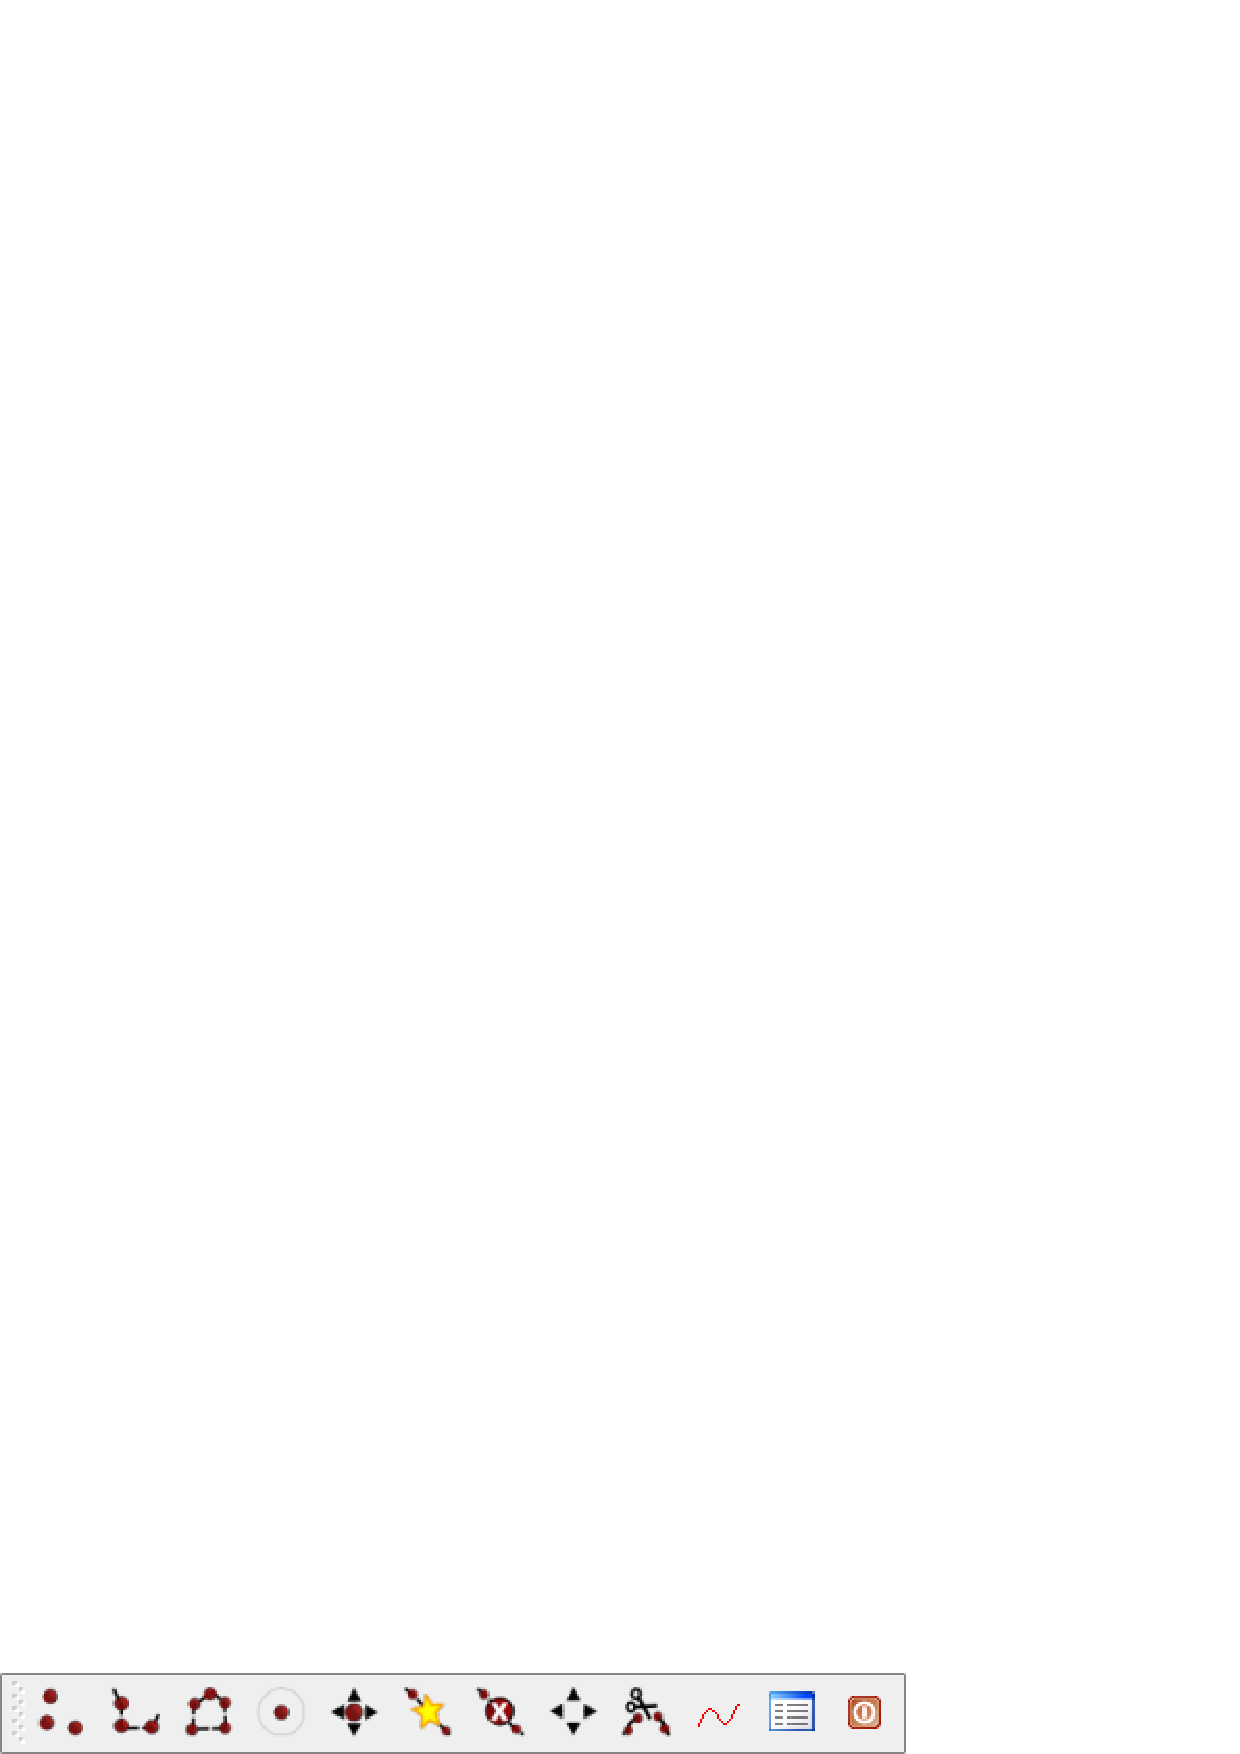
\includegraphics[clip=true,width=12cm]{grass_digitizing_toolbar}
\end{center}  
\end{figure}

\begin{table}[h]\index{GRASS!digitizing tools}
\centering
\caption{Strumenti per la digitalizzazione in GRASS}\label{tab:grass_tools}\medskip
 \begin{tabular}{|l|l|p{5in}|}
 \hline \textbf{Icone} & \textbf{Strumento} & \textbf{Scopo} \\
\hline 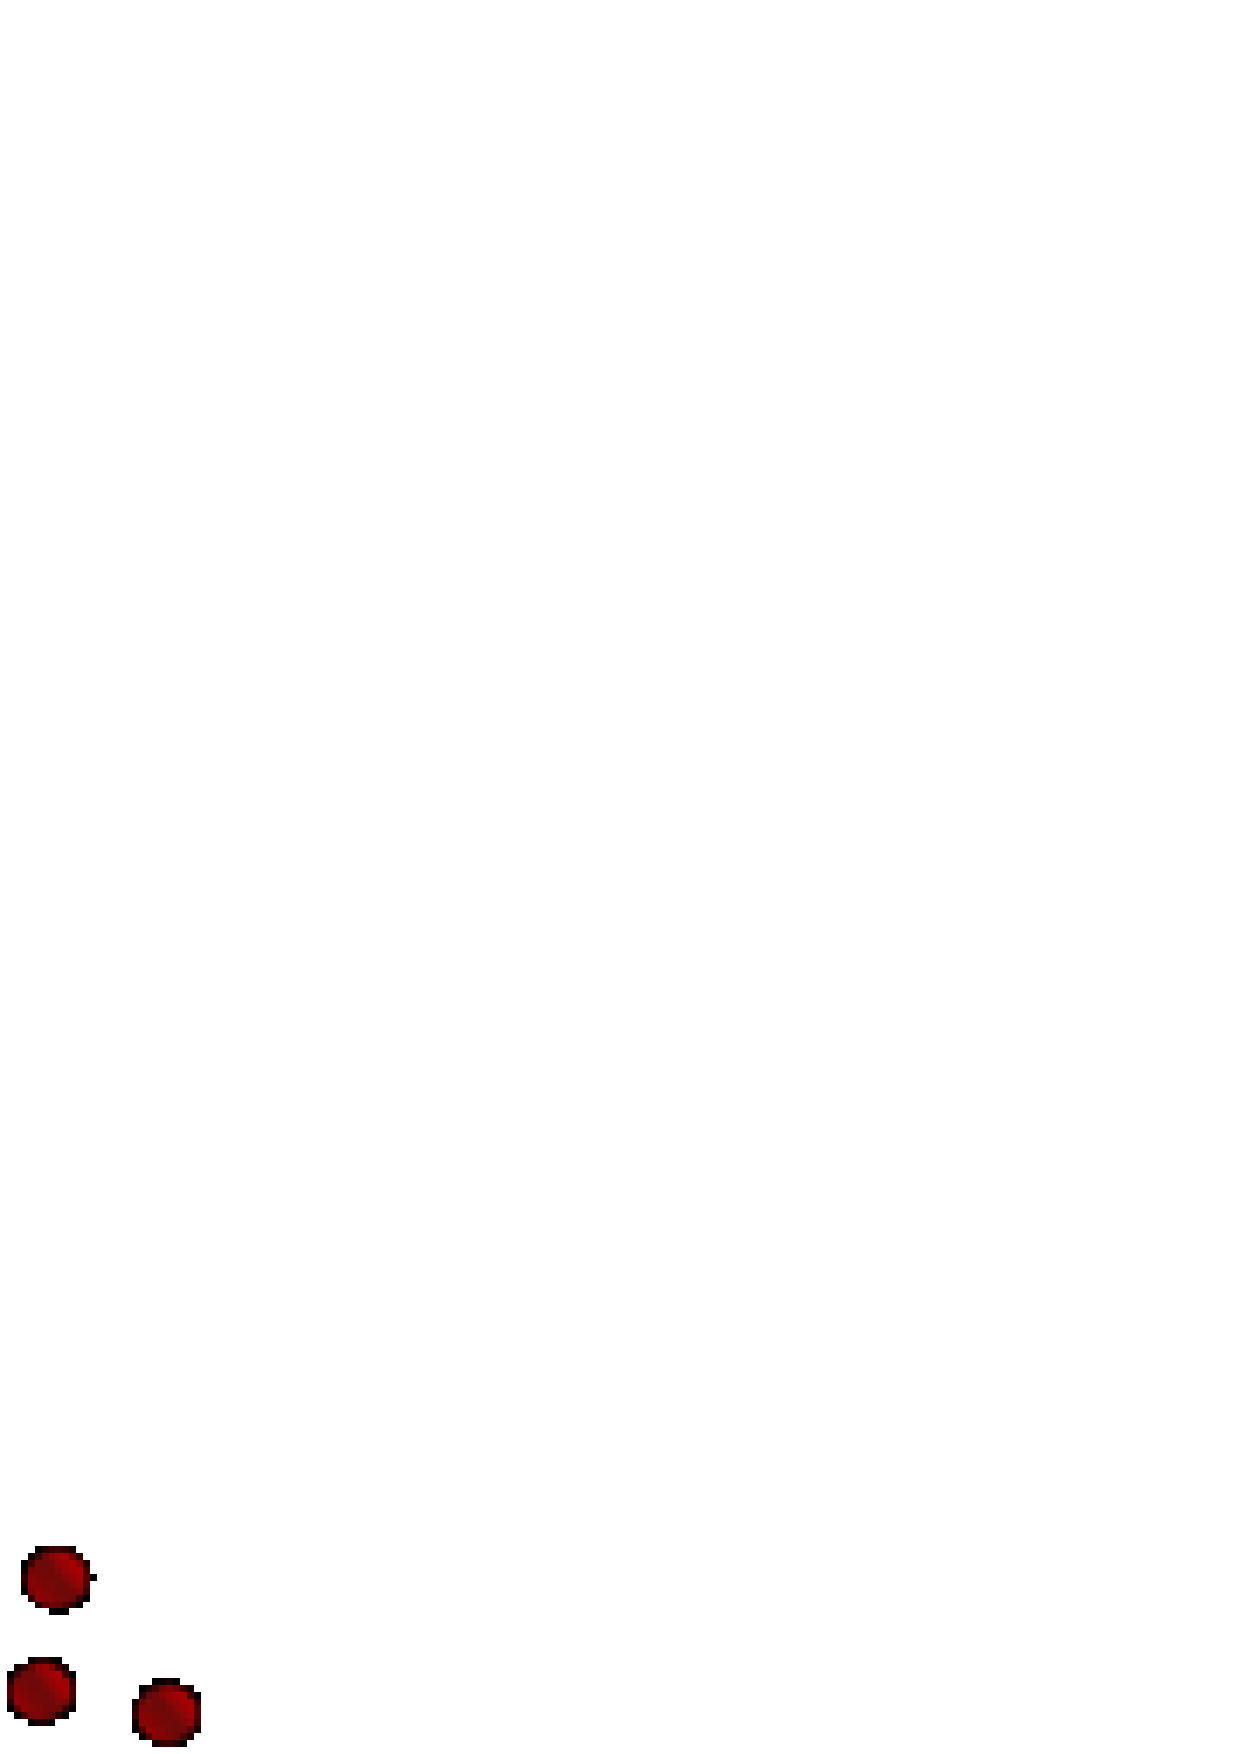
\includegraphics[width=0.7cm]{grass_new_point} & Nuovo punto &
Digitalizza un nuovo punto \\
\hline 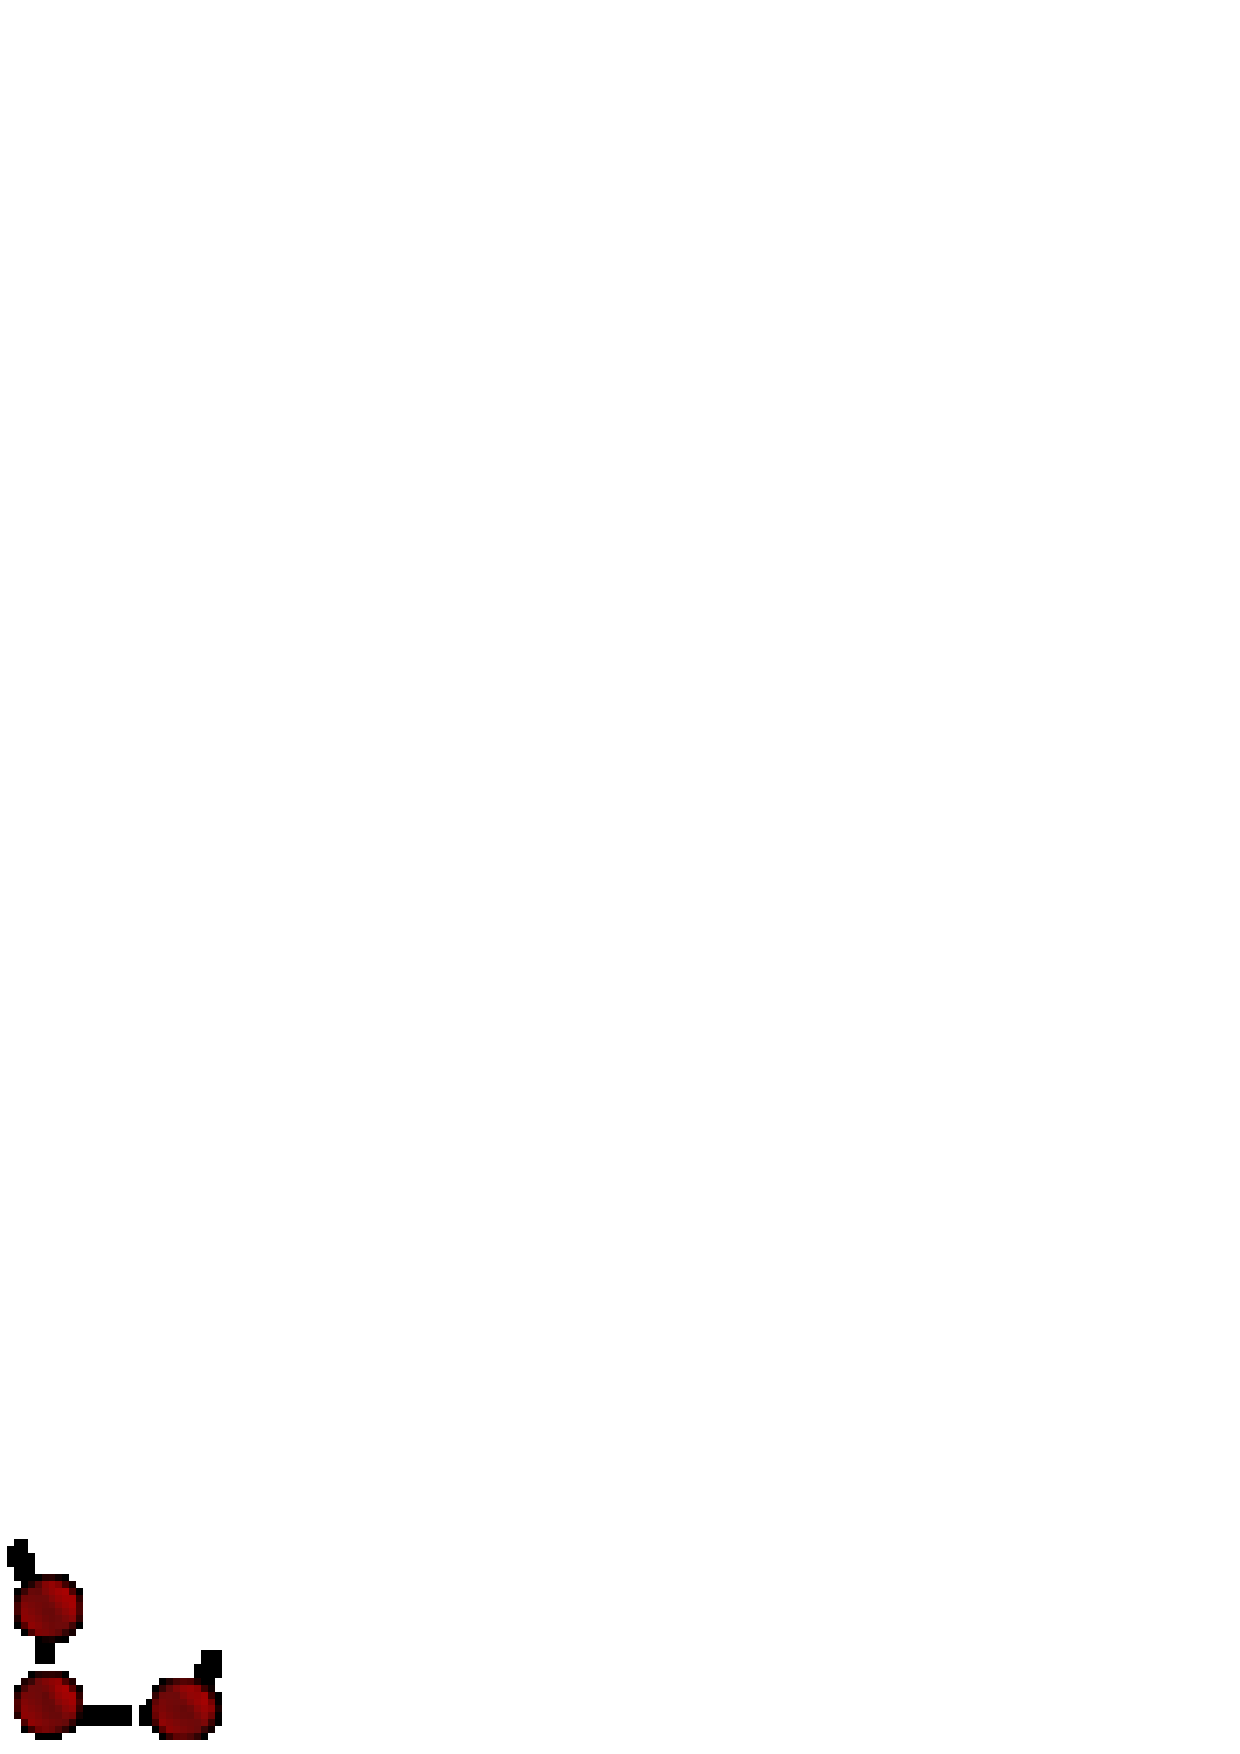
\includegraphics[width=0.7cm]{grass_new_line} & Nuova linea &
Digitalizza una nuova linea (annullare selezionando un altro strumento) \\
\hline 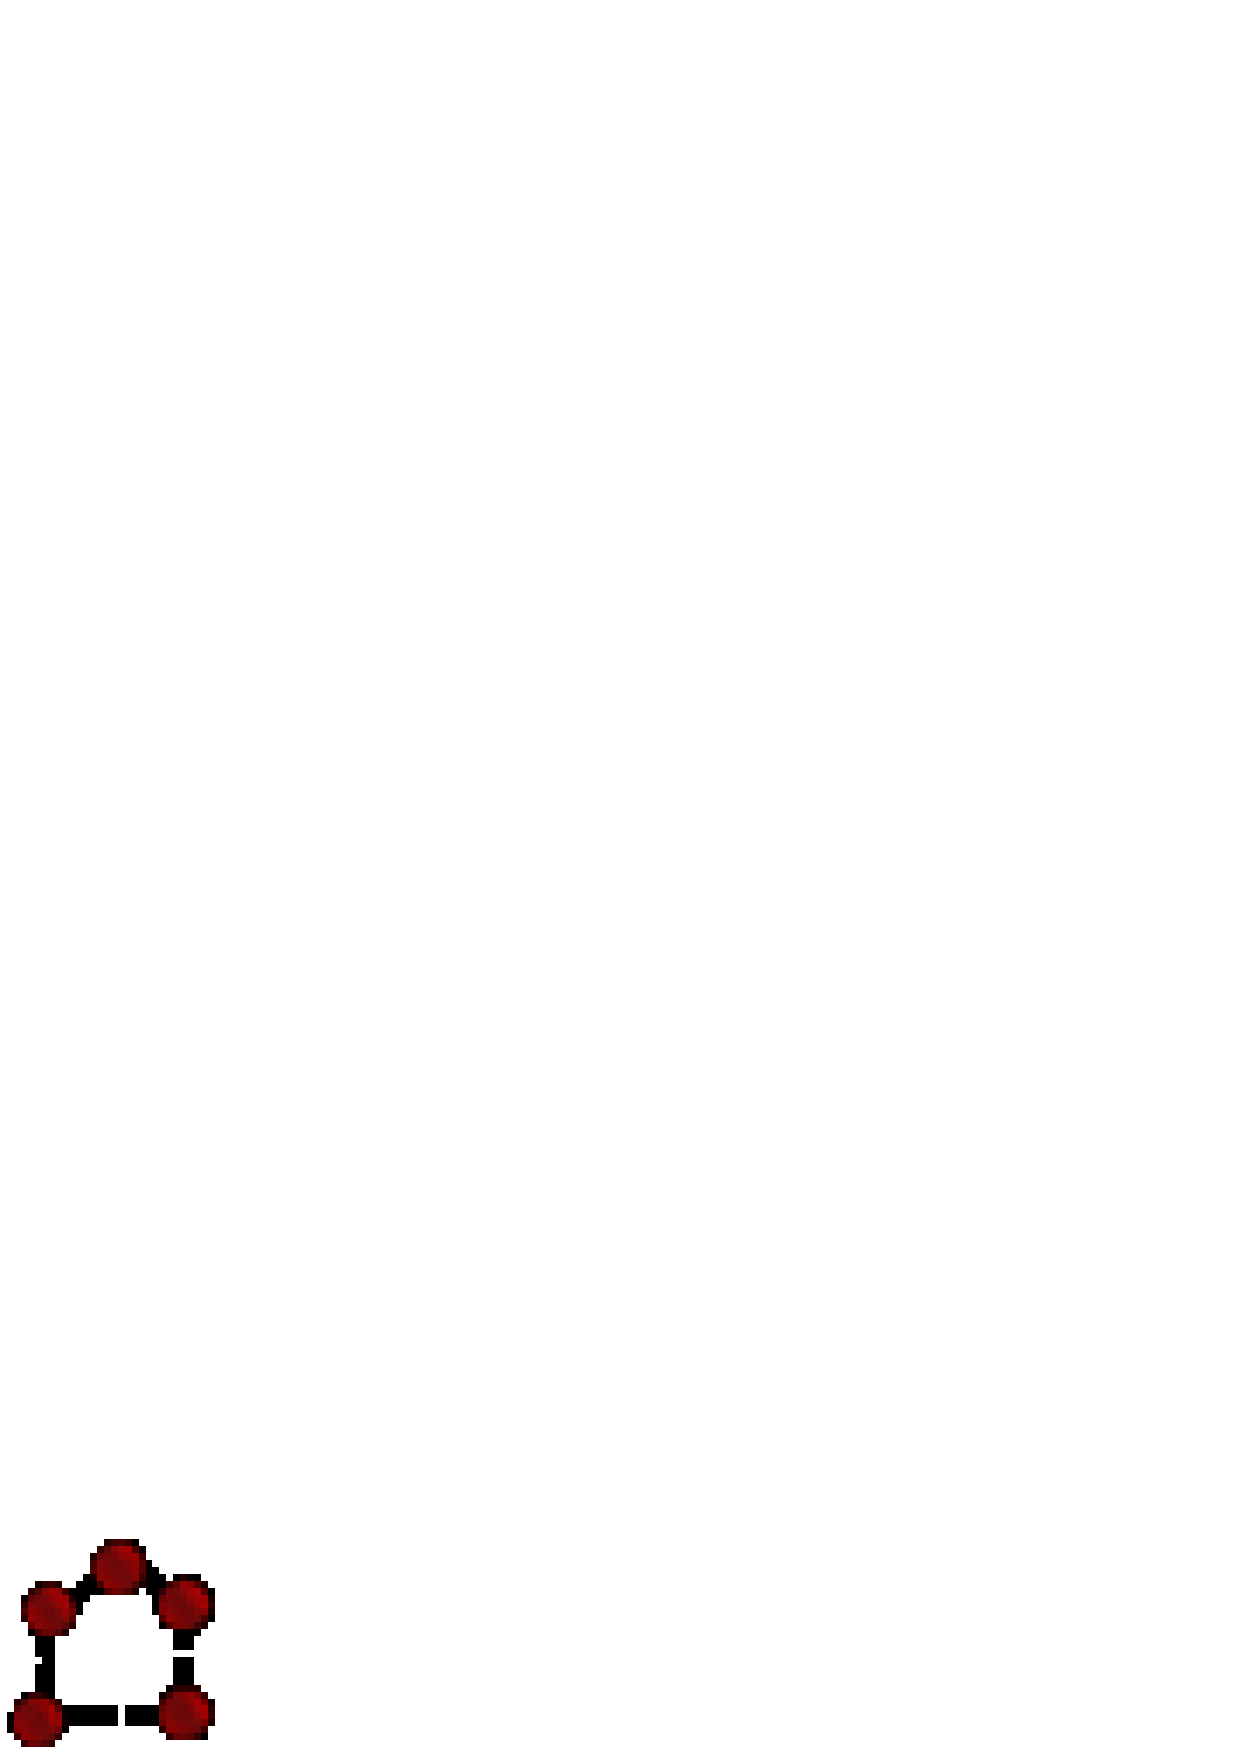
\includegraphics[width=0.7cm]{grass_new_boundary} & Nuovo contorno &
Digitizalizza nuovo contorno (annullare selezionando un altro strumento)\\
\hline 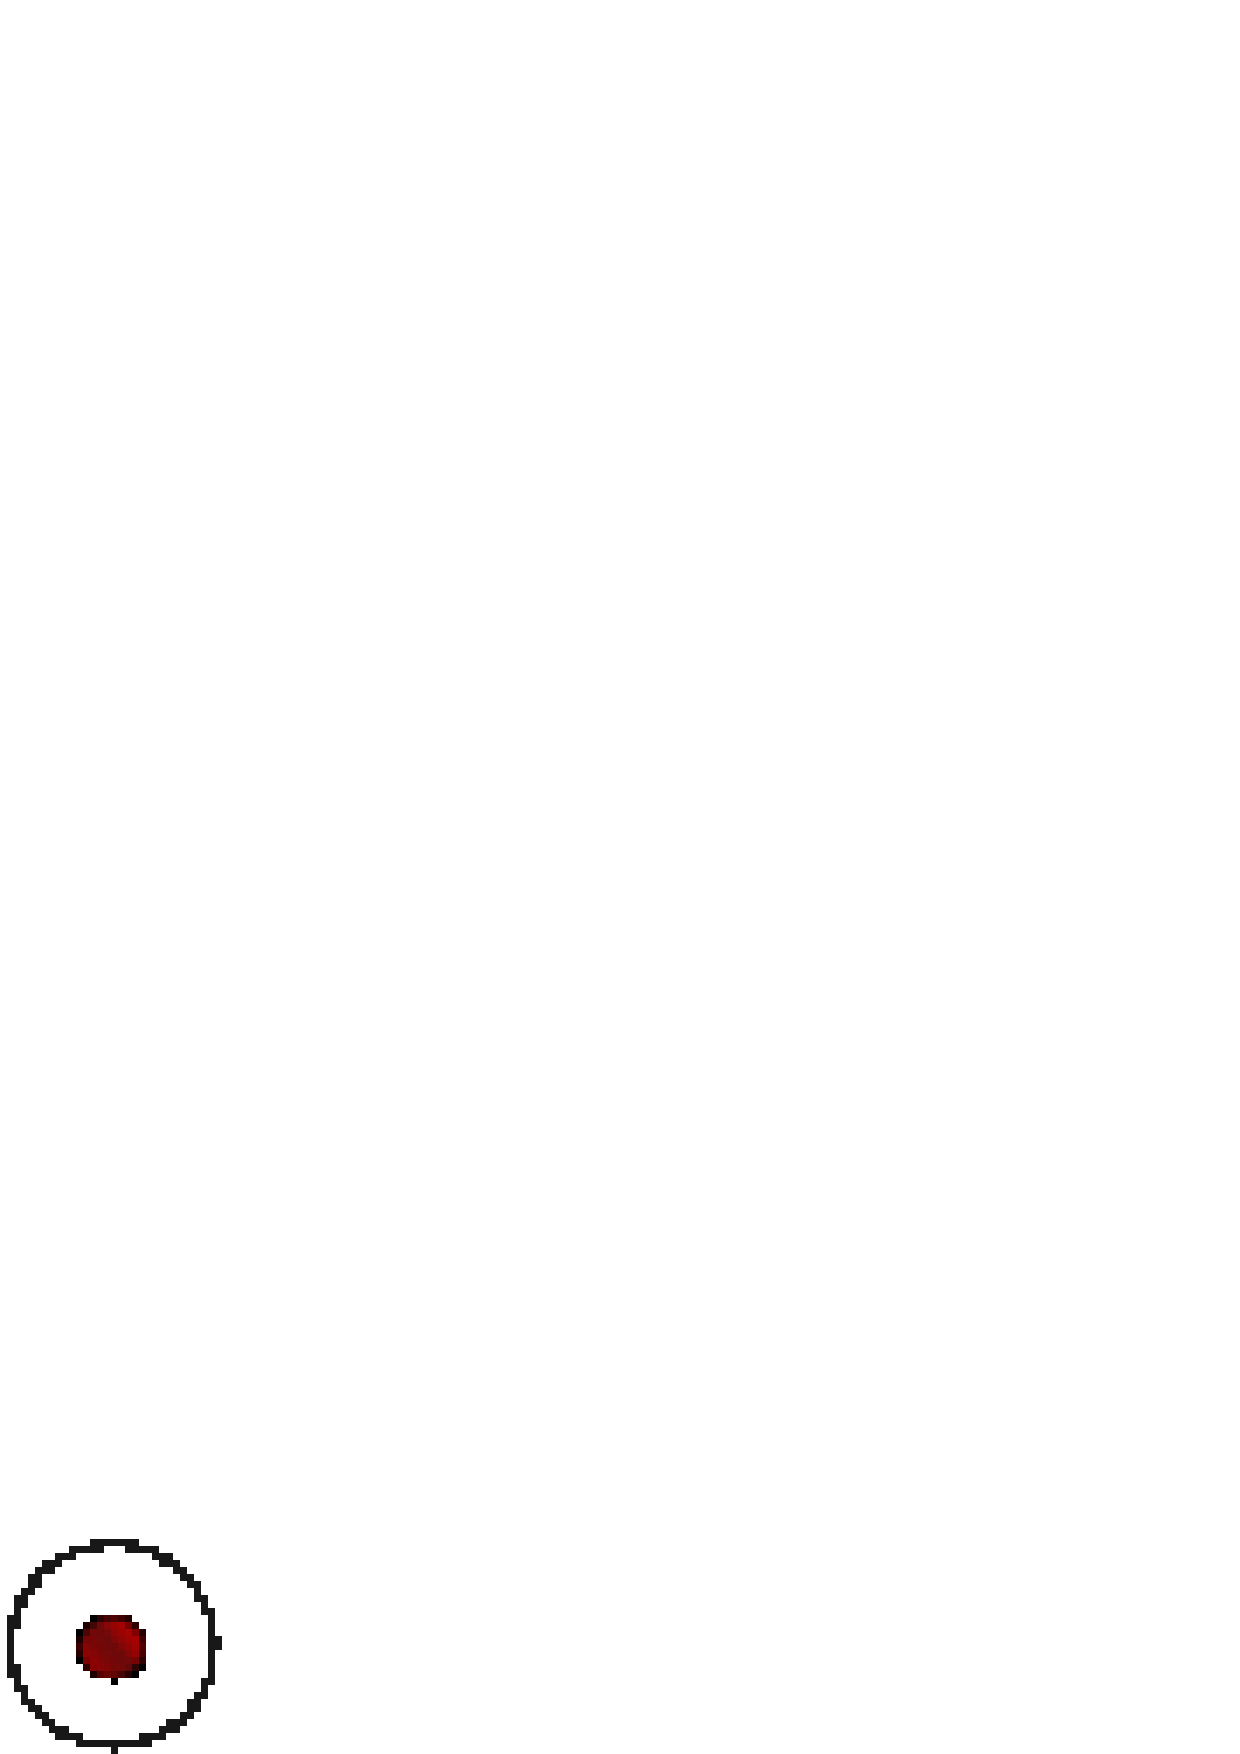
\includegraphics[width=0.7cm]{grass_new_centroid} & Nuovo centroide &
Digitalizza un nuovo centroide (imposta l'etichetta per area esitente)\\
\hline 
\includegraphics[width=0.7cm]{grass_move_vertex} & Sposta vertice &
Sposta un vertice di un'esistente linea o contorno in una nuova posizione\\
\hline 
\includegraphics[width=0.7cm]{grass_add_vertex} & Aggiungi vertice &
Aggiunge un vertice ad una linea o contorno esistente\\
\hline 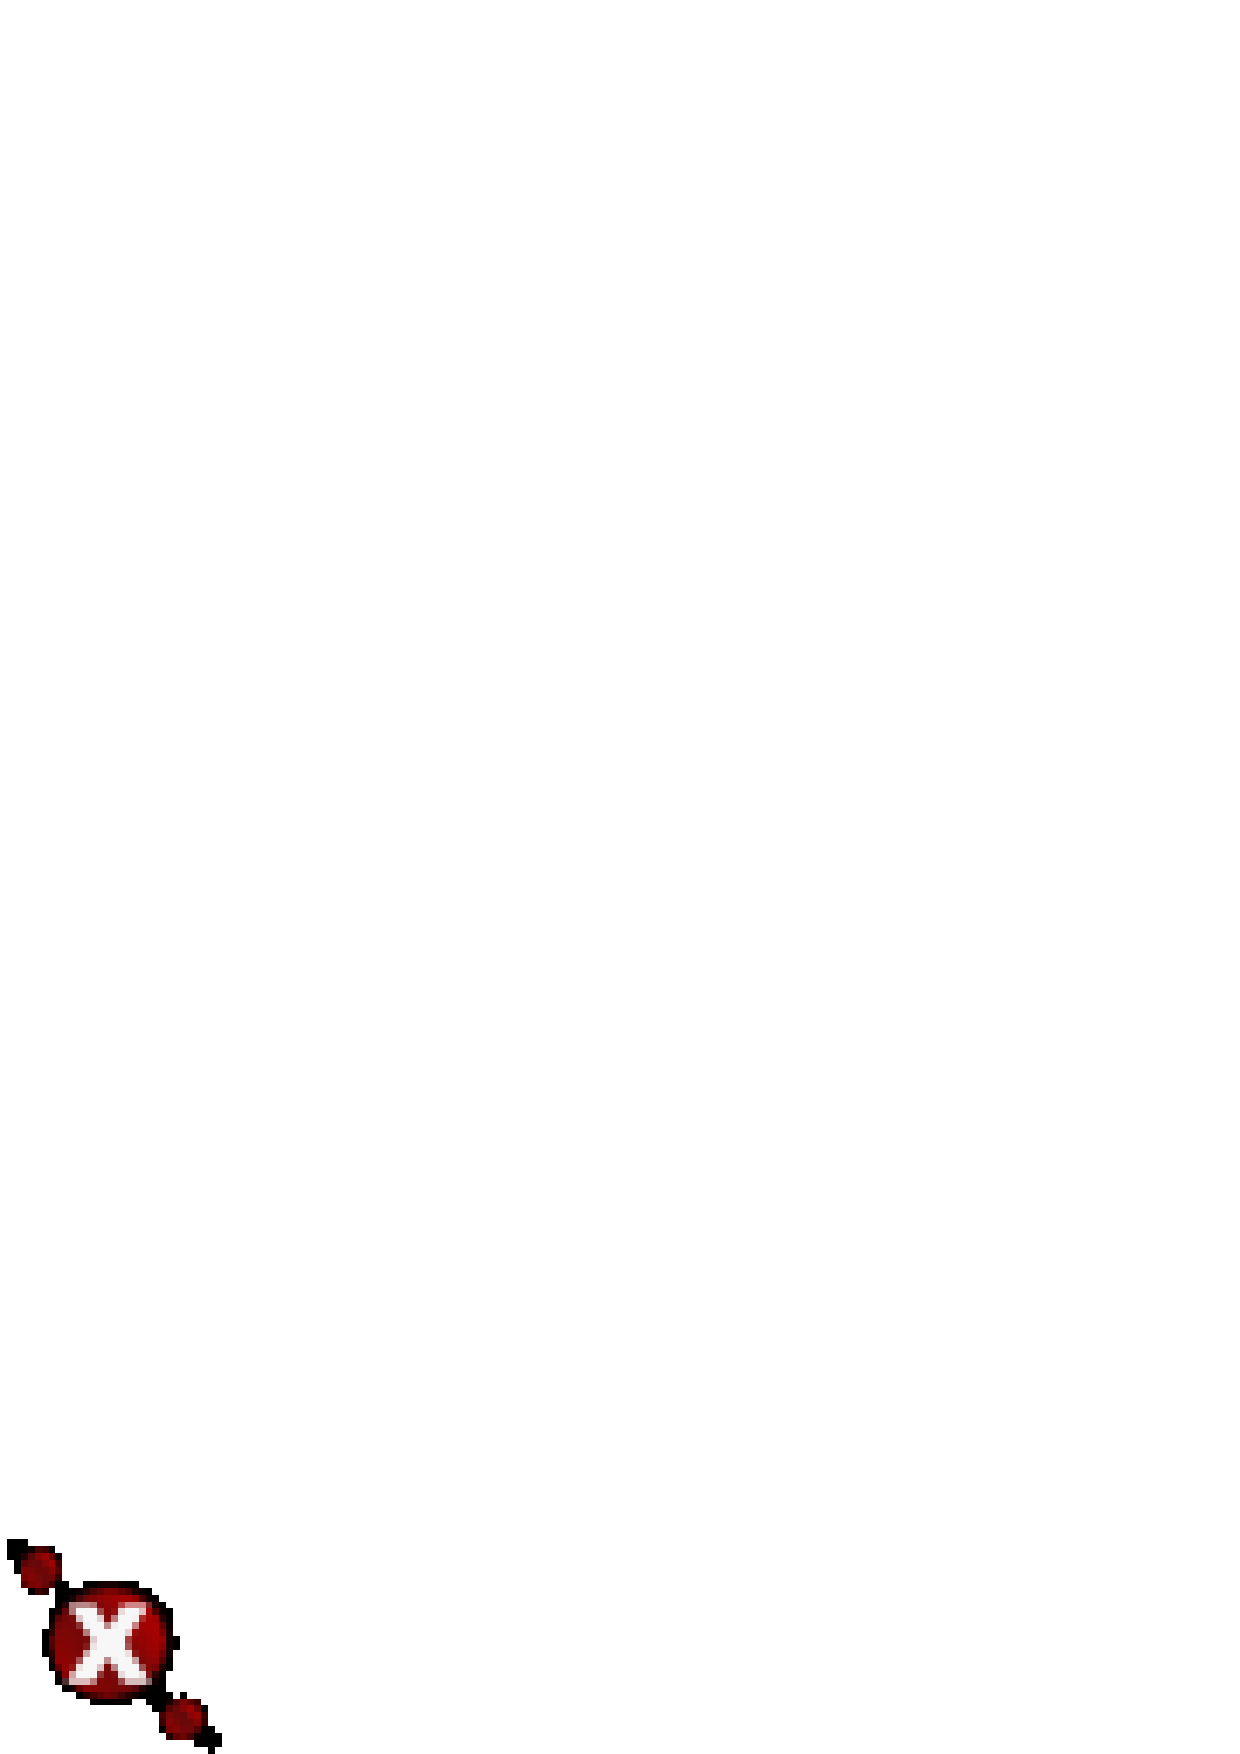
\includegraphics[width=0.7cm]{grass_delete_vertex} & Elimina vertice &
Cancella vertici da linee e contorni esistenti (confermare l'eliminazione del
vertice selezionato cliccando una seconda volta)\\
\hline 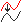
\includegraphics[width=0.7cm]{grass_move_line} & Sposta elemento &
Sposta il confine, la linea, il punto o il centroide selezionato in una nuova
posizione\\
\hline 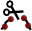
\includegraphics[width=0.7cm]{grass_split_line} & Dividi linea & Divide
una linea o un contorno in due parti nel punto selezionato (confermare
cliccando una seconda volta)\\
\hline 
\includegraphics[width=0.7cm]{grass_delete_line} & Elimina elemento &
Elimina un contorno, una linea, un punto o un centroide esistente (confermare
cliccando una seconda volta)\\
\hline 
\includegraphics[width=0.7cm]{grass_edit_attributes} & Modifica
attributi & Edita gli attributi dell'elemento selezionato (si noti che ad un
elemento possono essere associati più attributi, si veda sopra)\\
\hline 
\includegraphics[width=0.7cm]{grass_close_edit} & Chiudi & Chiudi la
sessione e salva lo stato attuale (ricostruisce conseguentemente la topologia)\\
\hline
\end{tabular}
\end{table}

\minisec{Scheda Categoria}\index{GRASS!impostazioni categoria}

La scheda \tab{Categoria} consente di definire il modo in cui i valori
della categoria verranno assegnati al nuovo elemento geometrico.

\begin{figure}[h]
 \begin{center}
  \caption{Scheda Categoria negli strumenti per la digitalizzazione in GRASS \nixcaption}\label{fig:grass_digitizing_category}
  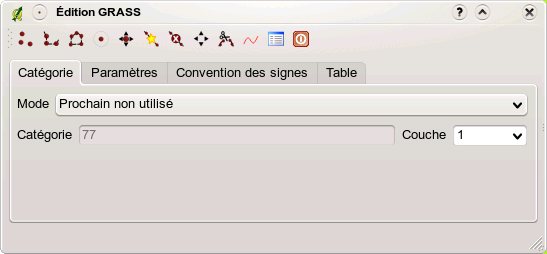
\includegraphics[clip=true,width=10cm]{grass_digitizing_category}
 \end{center}
\end{figure}

\begin{itemize}
\item \textbf{Modalità}: modalità con la quale viene assegnata la categoria
(colonna cat nella tabella) alle geometrie digitalizzate.
\begin{itemize}
\item Prossimo non in uso - applica il primo valore non utilizzato in ordine
numerico crescente all'elemento.
\item Inserimento manuale - definizione manuale della categoria da assegnare
all'elemento.
\item Nessuna categoria - non assegnare alcun valore all'elemento. Questa
modalità è in genere usata ad es. per i contorni dei poligoni ai quali la
categoria viene collegata tramite il centroide.
\end{itemize}
\item \textbf{Categoria} - Il numero (ID) inserito o visualizzato viene
associato ad ogni elemento digitalizzato. Viene usato per collegare ogni
elemento geometrico con i relativi attributi.
\item \textbf{Layer} - Ogni elemento geometrico può essere collegato
con molteplici tabelle attributo usando diversi "layer" secondo il
modello GRASS. Il layer di default è il numero 1. 
\end{itemize}

\begin{Tip}\caption{\textsc{Creare un "layer" GRASS aggiuntivo con QGIS}}
\qgistip{Se si vogliono aggiungere ulteriori layer al dato, inserire
semplicemente un numero nel campo "Layer" e dare invio. Nella scheda
Tabella sarà a questo punto possibile creare il nuovo schema degli attributi
da associare a questo "layer".
}
\end{Tip}

\minisec{Scheda Preferenze}\label{label_settingtab}\index{GRASS!tolleranza snap}

La scheda \tab{Preferenze} consente di impostare la tolleranza per
l'aggancio automatico tra elementi (snapping) in pixels dello schermo. La
soglia definisce a quale distanza massima nuovi punti o linee sono agganciati
ad altri nodi esistenti. Ciò aiuta ad evitare interruzioni o incroci tra
contorni. Il valore preimpostato è 10 pixels.

\begin{figure}[h]
 \begin{center}
 \caption{Scheda Preferenze negli strumenti per la digitalizzazione in GRASS \nixcaption}\label{fig:grass_digitizing_settings}
 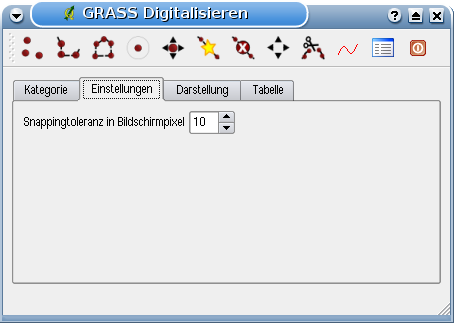
\includegraphics[clip=true,width=8cm]{grass_digitizing_settings}
 \end{center}
\end{figure}

\minisec{Scheda Simbologia}\index{GRASS!impostazioni simbologia}

La scheda \tab{Simbologia} consente di visualizzare e impostare la
simbologia e i colori dei vari tipi geometrici nei vari stati topologici (ad
es. contorni aperti/chiusi).

\begin{figure}[h]
 \begin{center}
 \caption{Scheda Simbologia negli strumenti per la digitalizzazione in GRASS \nixcaption}\label{fig:grass_digitizing_symbology}
 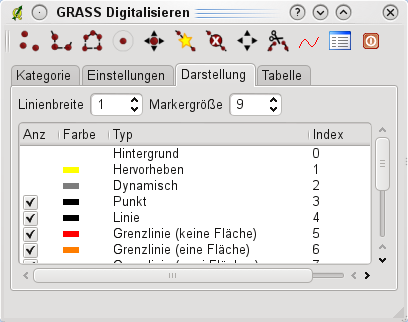
\includegraphics[clip=true,width=8cm]{grass_digitizing_symbology}
 \end{center}
\end{figure}

\minisec{Scheda Tabella} \index{GRASS!modifica tabella}

La scheda \tab{Tabella} fornisce informazioni sulla struttura della tabella
nel database per un determinato "layer". Qui si possono aggiungere nuove
colonne ad una tabella attributi esistente o creare un nuovo schema tabella
per un nuovo layer vettoriale GRASS o per un nuovo "layer" (si veda la Sezione 
\ref{sec:creating_new_grass_vectors}).

\begin{figure}[h]
 \begin{center}
 \caption{Scheda Tabella negli strumenti per la digitalizzazione in GRASS \nixcaption}\label{fig:grass_digitizing_table}
 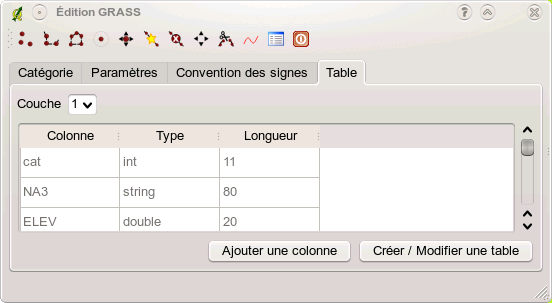
\includegraphics[clip=true,width=10cm]{grass_digitizing_table}
 \end{center}
\end{figure}

\begin{Tip}\caption{\textsc{Permessi di modifica in GRASS}}\index{GRASS!modifica permessi}
\qgistip{È necessario essere il proprietario del \filename{MAPSET} GRASS che
si vuole editare. Non è possibile modificare dati in un {MAPSET} del quale non
si è proprietari, anche se si possiedono si di esso permessi in scrittura.
}
\end{Tip} 

\subsection{Lo strumento Region di GRASS}\label{sec:grass_region}\index{GRASS!region}

L'impostazione di una regione (ovvero di una porzione di spazio geografico
nella quale operare) è molto importante in GRASS quando si lavora con dati
raster. L'analisi vettoriale infatti di default non è limitata
dall'impostazione della regione ma viene fatta su tutta l'estensione del
layer. Tutti i raster di nuova creazione avranno l'estensione e risoluzione
spaziale della regione GRASS definita, indipendentemente dalla loro estensione
e risoluzione originale. L'impostazione corrente della regione GRASS è salvata
nel file \filename{\$LOCATION/\$MAPSET/WIND} che ne definisce i limiti nord, sud
est e ovest, il numero di righe e colonne e la risoluzione spaziale in senso
orizzontale e verticale.

È possibile abilitare/disabilitare la visualizzazione della region di GRASS
nella vista mappa in QGIS usando il pulsante \toolbtntwo{grass_region}{Visualizza GRASS regione attuale}. \index{GRASS!region!visualizza}.

Con lo strumento \toolbtntwo{grass_region_edit}{Modifica region GRASS attuale}
è possibile aprire una finestra di dialogo per cambiare le impostazioni
attuali della regione e la simbologia con la quale il rettangolo che la
rappresenta viene visualizzato nella vista mappa di QGIS. Inserire i nuovi
limiti della regione e la risoluzione e cliccare su \button{OK}. Lo strumento
consente anche di selezionare l'estensione della regione interattivamente con
il mouse nella vista mappa di QGIS. Cliccando quindi con il tasto sinistro del
mouse nella vista mappa si imposta il primo angolo del rettangolo che definirà
la regione e cliccando in un altro punto lo si chiuderà. Cliccare quindi su
\button{OK} per confermare.\index{GRASS!region!modifica}
Il modulo GRASS \filename{g.region} mette a disposizione molti più parametri
per definire l'estensione della regione e la risoluzione con la quale si vuole
condurre l'analisi raster. Si possono usare questi parametri usando lo
strumento appropriato nella barra GRASS, descritta nella Sezione \ref{subsec:grass_toolbox}.

\subsection{La barra strumenti GRASS}\label{subsec:grass_toolbox}\index{GRASS!strumenti}

Lo strumento \toolbtntwo{grass_tools}{Apri strumenti GRASS} fornisce accesso
alle funzionalità dei moduli GRASS con i quali lavorare nella
\filename{LOCATION} e nel \filename{MAPSET} impostati. Per usare gli strumenti
di GRASS è necessario aprire una \filename{LOCATION} e un \filename{MAPSET}
sui quali si abbiano permessi di scrittura (in genere concessi se si è
l'utente che ha creato il \filename{MAPSET}). Ciò è necessario in quanto i
nuovi layer raster o vettoriali creati durante l'analisi devono poter essere
scritti nella \filename{LOCATION} e nel \filename{MAPSET} selezionato.

\subsubsection{Lavorare con i moduli GRASS}\index{GRASS!strumenti}

\begin{figure}[h]
\centering
\caption{Strumenti di GRASS e Lista Moduli con possibilità di ricerca \nixcaption}\label{fig:grass_modules}
   \subfigure[Albero moduli] {\label{subfig:grass_module_tree}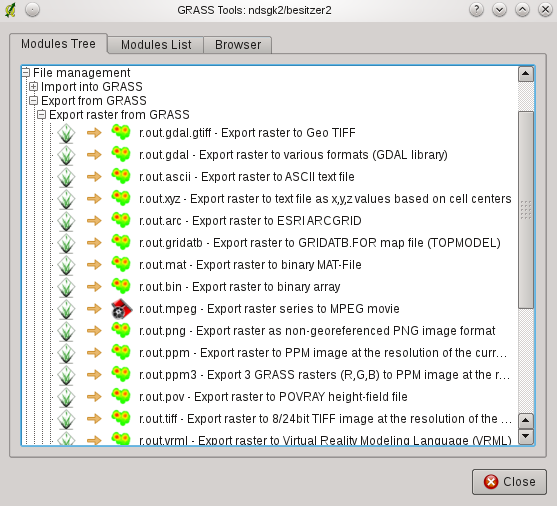
\includegraphics[clip=true, width=0.4\textwidth]{grass_toolbox_moduletree}}\goodgap
   \subfigure[Lista moduli con casella di ricerca] {\label{subfig:grass_module_list}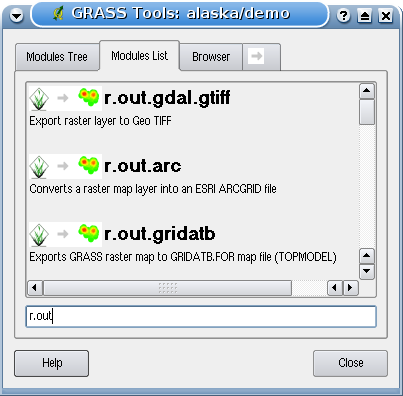
\includegraphics[clip=true, width=0.4\textwidth]{grass_toolbox_modulelist}}
\end{figure}

La shell di GRASS negli strumenti fornisce accesso a praticamente tutti gli
oltre 300 moduli GRASS in modalità riga di comando. Per offrire un ambiente di
lavoro maggiormente user-friendly, circa 200 di questi moduli e delle relative
funzionalità sono presentate in finestre di dialogo. Questi moduli sono
raggruppate in blocchi tematici ma possono anche essere cercati. Una lista
completa dei moduli GRASS disponibili nella versione di QGIS \CURRENT
è fornita in Appendice \ref{appdx_grass_toolbox_modules}. È anche possibile
personalizzare il contenuto degli strumenti GRASS come descritto alla Sezione 
\ref{sec:toolbox-customizing}.

Come mostrato in Figura \ref{fig:grass_modules}, è possibile cercare il modulo
GRASS desiderato cercandolo per aree tematiche nella scheda \tab{Albero
moduli} o nella scheda con casella di ricerca \tab{Lista moduli}. 

Cliccando sull'icona di un modulo grafico verrà aggiunta una nuova scheda
alla finestra degli strumenti. In questa scheda si avranno tre ulteriori
sottoschede denominate \tab{Opzioni}, \tab{Output} e \tab{Manuale}. Un
esempio è mostrato in Figura \ref{fig:grass_module_dialog} per il modulo
\filename{v.buffer}.

\begin{figure}[h]
\centering
\caption{Finestre degli strumenti GRASS \nixcaption}\label{fig:grass_module_dialog}
   \subfigure[Scheda Opzioni] {\label{subfig:grass_module_option}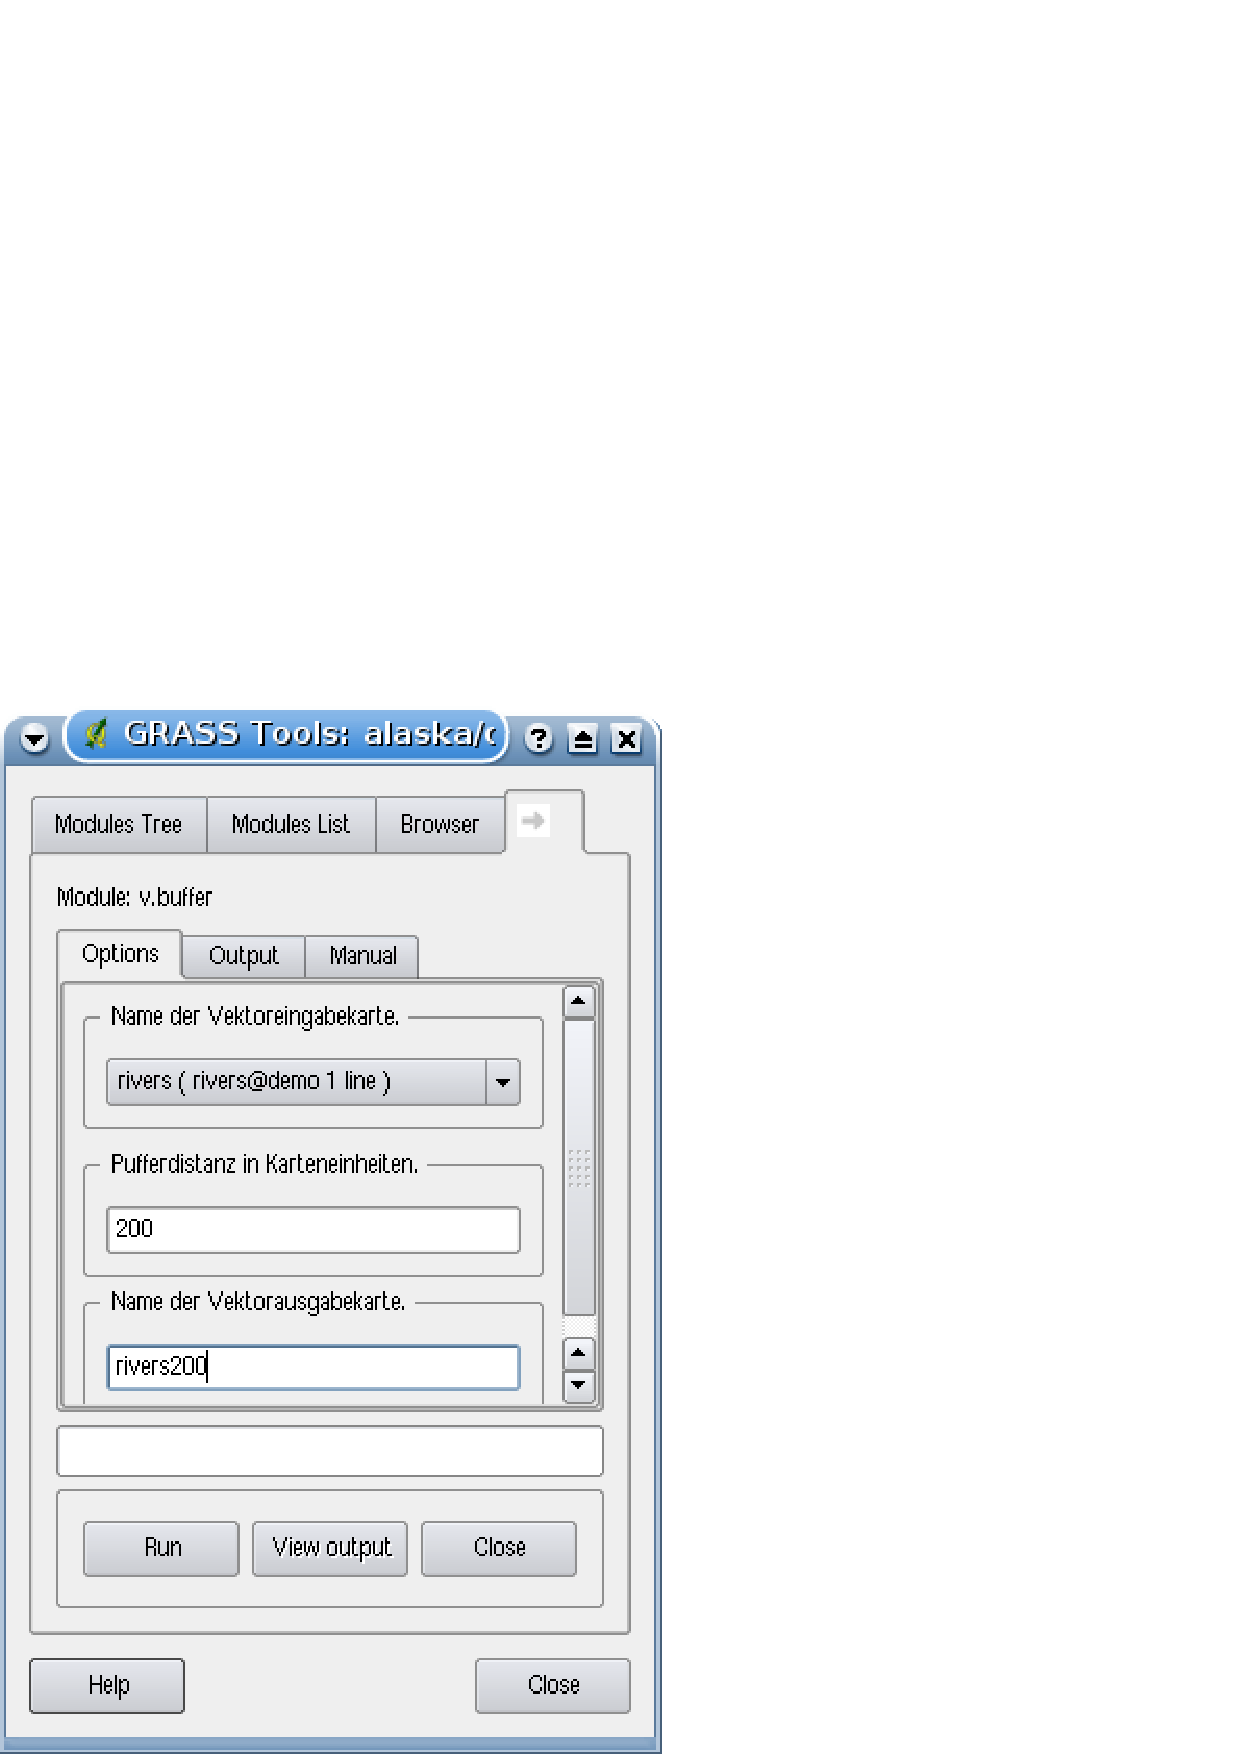
\includegraphics[clip=true, width=0.3\textwidth]{grass_module_option}}\goodgap
   \subfigure[Scheda Output] {\label{subfig:grass_module_output}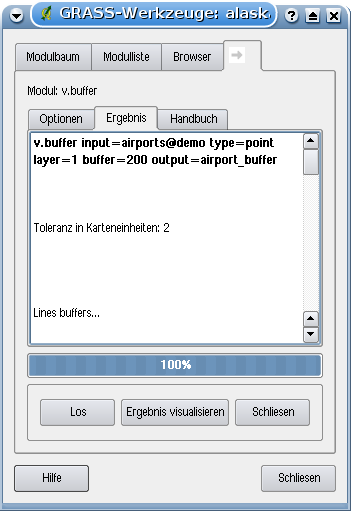
\includegraphics[clip=true, width=0.3\textwidth]{grass_module_output}}\goodgap
   \subfigure[Scheda Manuale] {\label{subfig:grass_module_manual}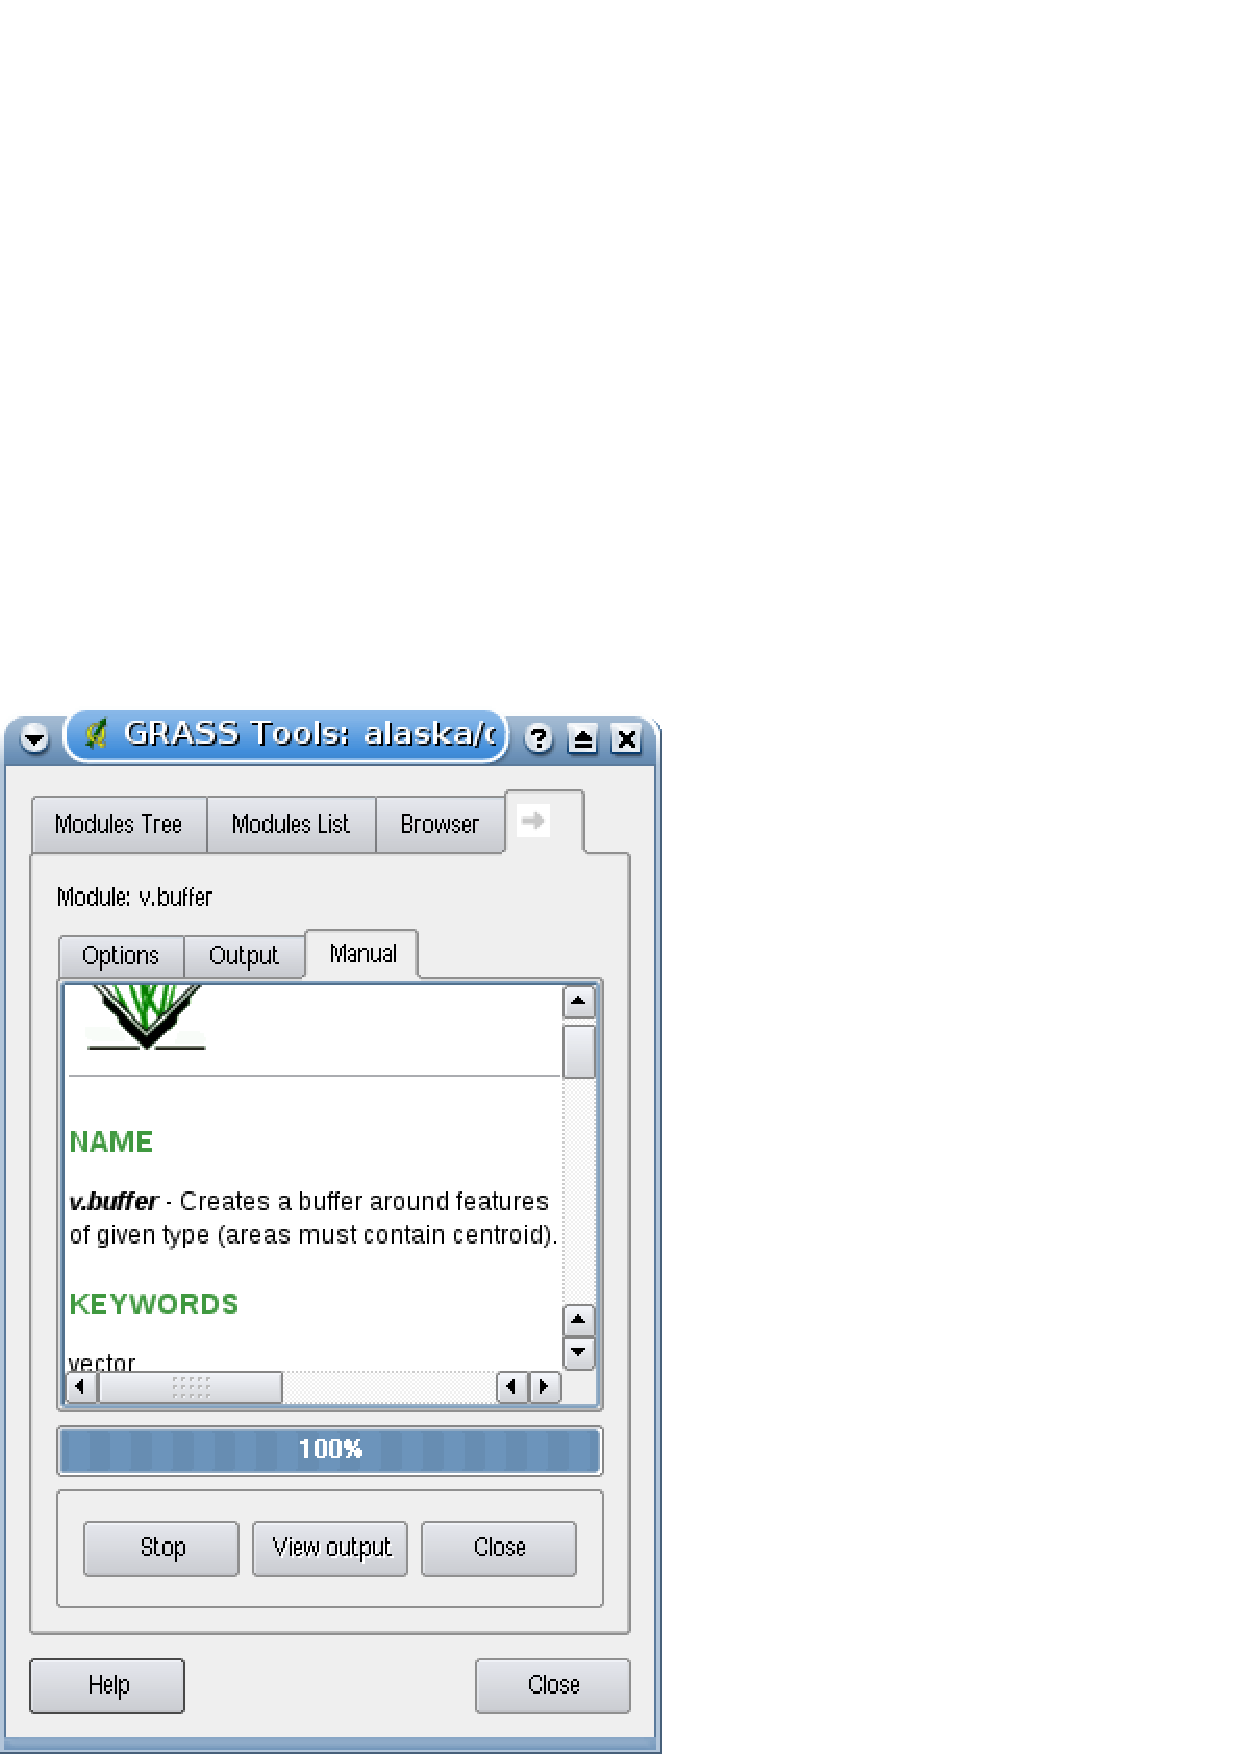
\includegraphics[clip=true, width=0.3\textwidth]{grass_module_manual}}
\end{figure}

\minisec{Opzioni}

La scheda \tab{Opzioni} fornisce una finestra semplificata nel quale di
solito è possibile selezionare un layer raster o vettoriale ed inserire
ulteriori opzioni specifiche per l'esecuzione del modulo. Per mantenere la
leggibilità della finestra non sempre sono presenti tutte le opzioni, se si
volessero usare ulteriori parametri per il modulo è necessario avviare la
shell di GRASS e eseguire il modulo dalla riga di comando.

\minisec{Output}

La scheda \tab{Output} fornisce informazioni sull'avanzamento delle
operazioni eseguite dal modulo. Quando si clicca sul pulsante \button{Esegui},
viene portata in primo piano la scheda \tab{Output} nella quale vengono
visualizzate le informazioni sul processo in corso. Se l'operazione va a buon
fine, si vedrà il messaggio \usertext{Operazione conclusa con successo}.

\minisec{Manuale}

La scheda \tab{Manual} mostra la pagina di aiuto in formato HTML del modulo
GRASS scelto. Qui può essere controllata la disponibilità di ulteriori
parametri o ottenere una conoscenza più approfondita sulle operazioni che il
modulo può eseguire. Ala fine di ogni pagina di manuale vi sono ulteriori
collegamenti al \filename{Main Help index}, al \filename{Thematic index} o al
\filename{Full index}. Questi link forniscono le stesse informazioni che si
avrebbero usando il modulo \filename{g.manual}.

\begin{Tip}\caption{\textsc{Mostrare i risultati immediatamente}}\index{GRASS!visualizza risultato}
\qgistip{Se si desidera visualizzare il risultato dell'analisi immediatamente
nella vista mappa, è possibile cliccare sul pulsante "Visualizza Output" nella
porzione inferiore della scheda.
}
\end{Tip} 

\subsubsection{Lavorare con il browser delle LOCATION GRASS} \index{GRASS!strumenti!browser}

Un'altra utile funzione tra quelle presenti negli strumenti GRASS è il browser
delle \filename{LOCATION}. In Figura~\ref{fig:grass_mapset_browser} è
possibile vedere un esempio che mostra la \filename{LOCATION} impostata 
e i relativi \filename{MAPSETs}.

Nella parte sinistra della finestra del browser si può navigare attraverso
tutti i \filename{MAPSETs} contenuti nella \filename{LOCATION} impostata. La
porzione di destra mostra invece alcuni metadati del raster o del vettoriale
selezionato, come la risoluzione, l'estensione spaziale, la fonte del dato, il
percorso alla tabella attributi associata per i dati vettoriali e lo storico
comandi che ha generato quel dato.

\begin{figure}[h]
 \begin{center}
 \caption{Browser delle LOCATION GRASS \nixcaption}\label{fig:grass_mapset_browser}
 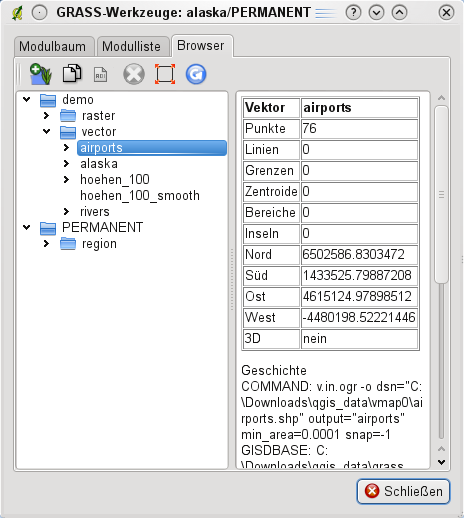
\includegraphics[clip=true,width=10cm]{grass_mapset_browser}
 \end{center}
\end{figure}

La barra strumenti nella scheda \tab{Browser} tab offre i seguenti
strumenti per la gestione della \filename{LOCATION} selezionata:

\begin{itemize}
\item \toolboxtwo{grass_add_map}{Aggiungi la mappa selezionata all'area di
lavoro}
\item \toolboxtwo{grass_copy_map}{Copia la mappa selezionata}
\item \toolboxtwo{grass_rename_map}{Rinomina la mappa selezionata}
\item \toolboxtwo{grass_delete_map}{Elimina la mappa selezionata}
\item \toolboxtwo{grass_set_region}{Imposta la regione corrente con la mappa
selezionata}
\item \toolboxtwo{grass_refresh}{Aggiorna}
\end{itemize}

Gli strumenti \toolboxtwo{grass_rename_map}{Rinomina la mappa selezionata} e
\toolboxtwo{grass_delete_map}{Elimina la mappa selezionata} funzionano solo su
mappe contenute nel \filename{MAPSET} attivo. Tutti gli altri strumenti
funzionano anche con layer raster e vettoriali di altri \filename{MAPSET}.

\subsubsection{Personalizzazione degli strumenti GRASS} \index{GRASS!strumenti!personalizza}
\label{sec:toolbox-customizing}

Praticamente tutti i moduli GRASS possono essere aggiunti agli strumenti
GRASS. Per incorporare i file XML di configurazione dei moduli è fornita
un'interfaccia XML nella quale definire l'aspetto del modulo e i parametri
da visualizzare nello strumento.

Un esempio di file XML che genera il modulo \usertext{v.buffer} (v.buffer.qgm)
ha il seguente aspetto:

\begin{verbatim}
<?xml version="1.0" encoding="UTF-8"?>
<!DOCTYPE qgisgrassmodule SYSTEM "http://mrcc.com/qgisgrassmodule.dtd">

<qgisgrassmodule label="Vector buffer" module="v.buffer">
        <option key="input" typeoption="type" layeroption="layer" />
        <option key="buffer"/>
        <option key="output" />
</qgisgrassmodule>
\end{verbatim}

Il parser legge questa definizione e crea una nuova scheda negli strumenti
quando si seleziona il modulo. Informazioni più dettagliate su come aggiungere
moduli, cambiare i gruppi di moduli ecc. sono reperibile sul Wiki di QGIS
all'indirizzo \\
\url{http://wiki.qgis.org/qgiswiki/Adding\_New\_Tools\_to\_the\_GRASS\_Toolbox}.

